\documentclass[11pt,a4paper,fleqn,titlepage,twoside,openany,export]{book}
\usepackage{style}

\subfile{05-slovnik-pojmu}

\bibliography{bibliography}


\begin{document}

\makeatletter
\begin{titlepage}
	\begin{center}
	
	\textsc{\Huge{Univerzita Pardubice}}

	\LARGE{Fakulta elektrotechniky a informatiky}
	
	\vfill
	
	\huge{\@title}\\[2mm]
	\LARGE{\@author}
	
	\vfill

	\begin{normalsize}
	Diplomová práce\\
	2015
	\end{normalsize}
	\end{center}
\end{titlepage}


\newpage  
\thispagestyle{empty}
\begin{center}

\includegraphics[max width=\textwidth,keepaspectratio=true]{imgs-00-zadani/zadani_str_1.png}
\end{center}
\hspace{0pt}

\newpage 
\thispagestyle{empty}
\begin{center}
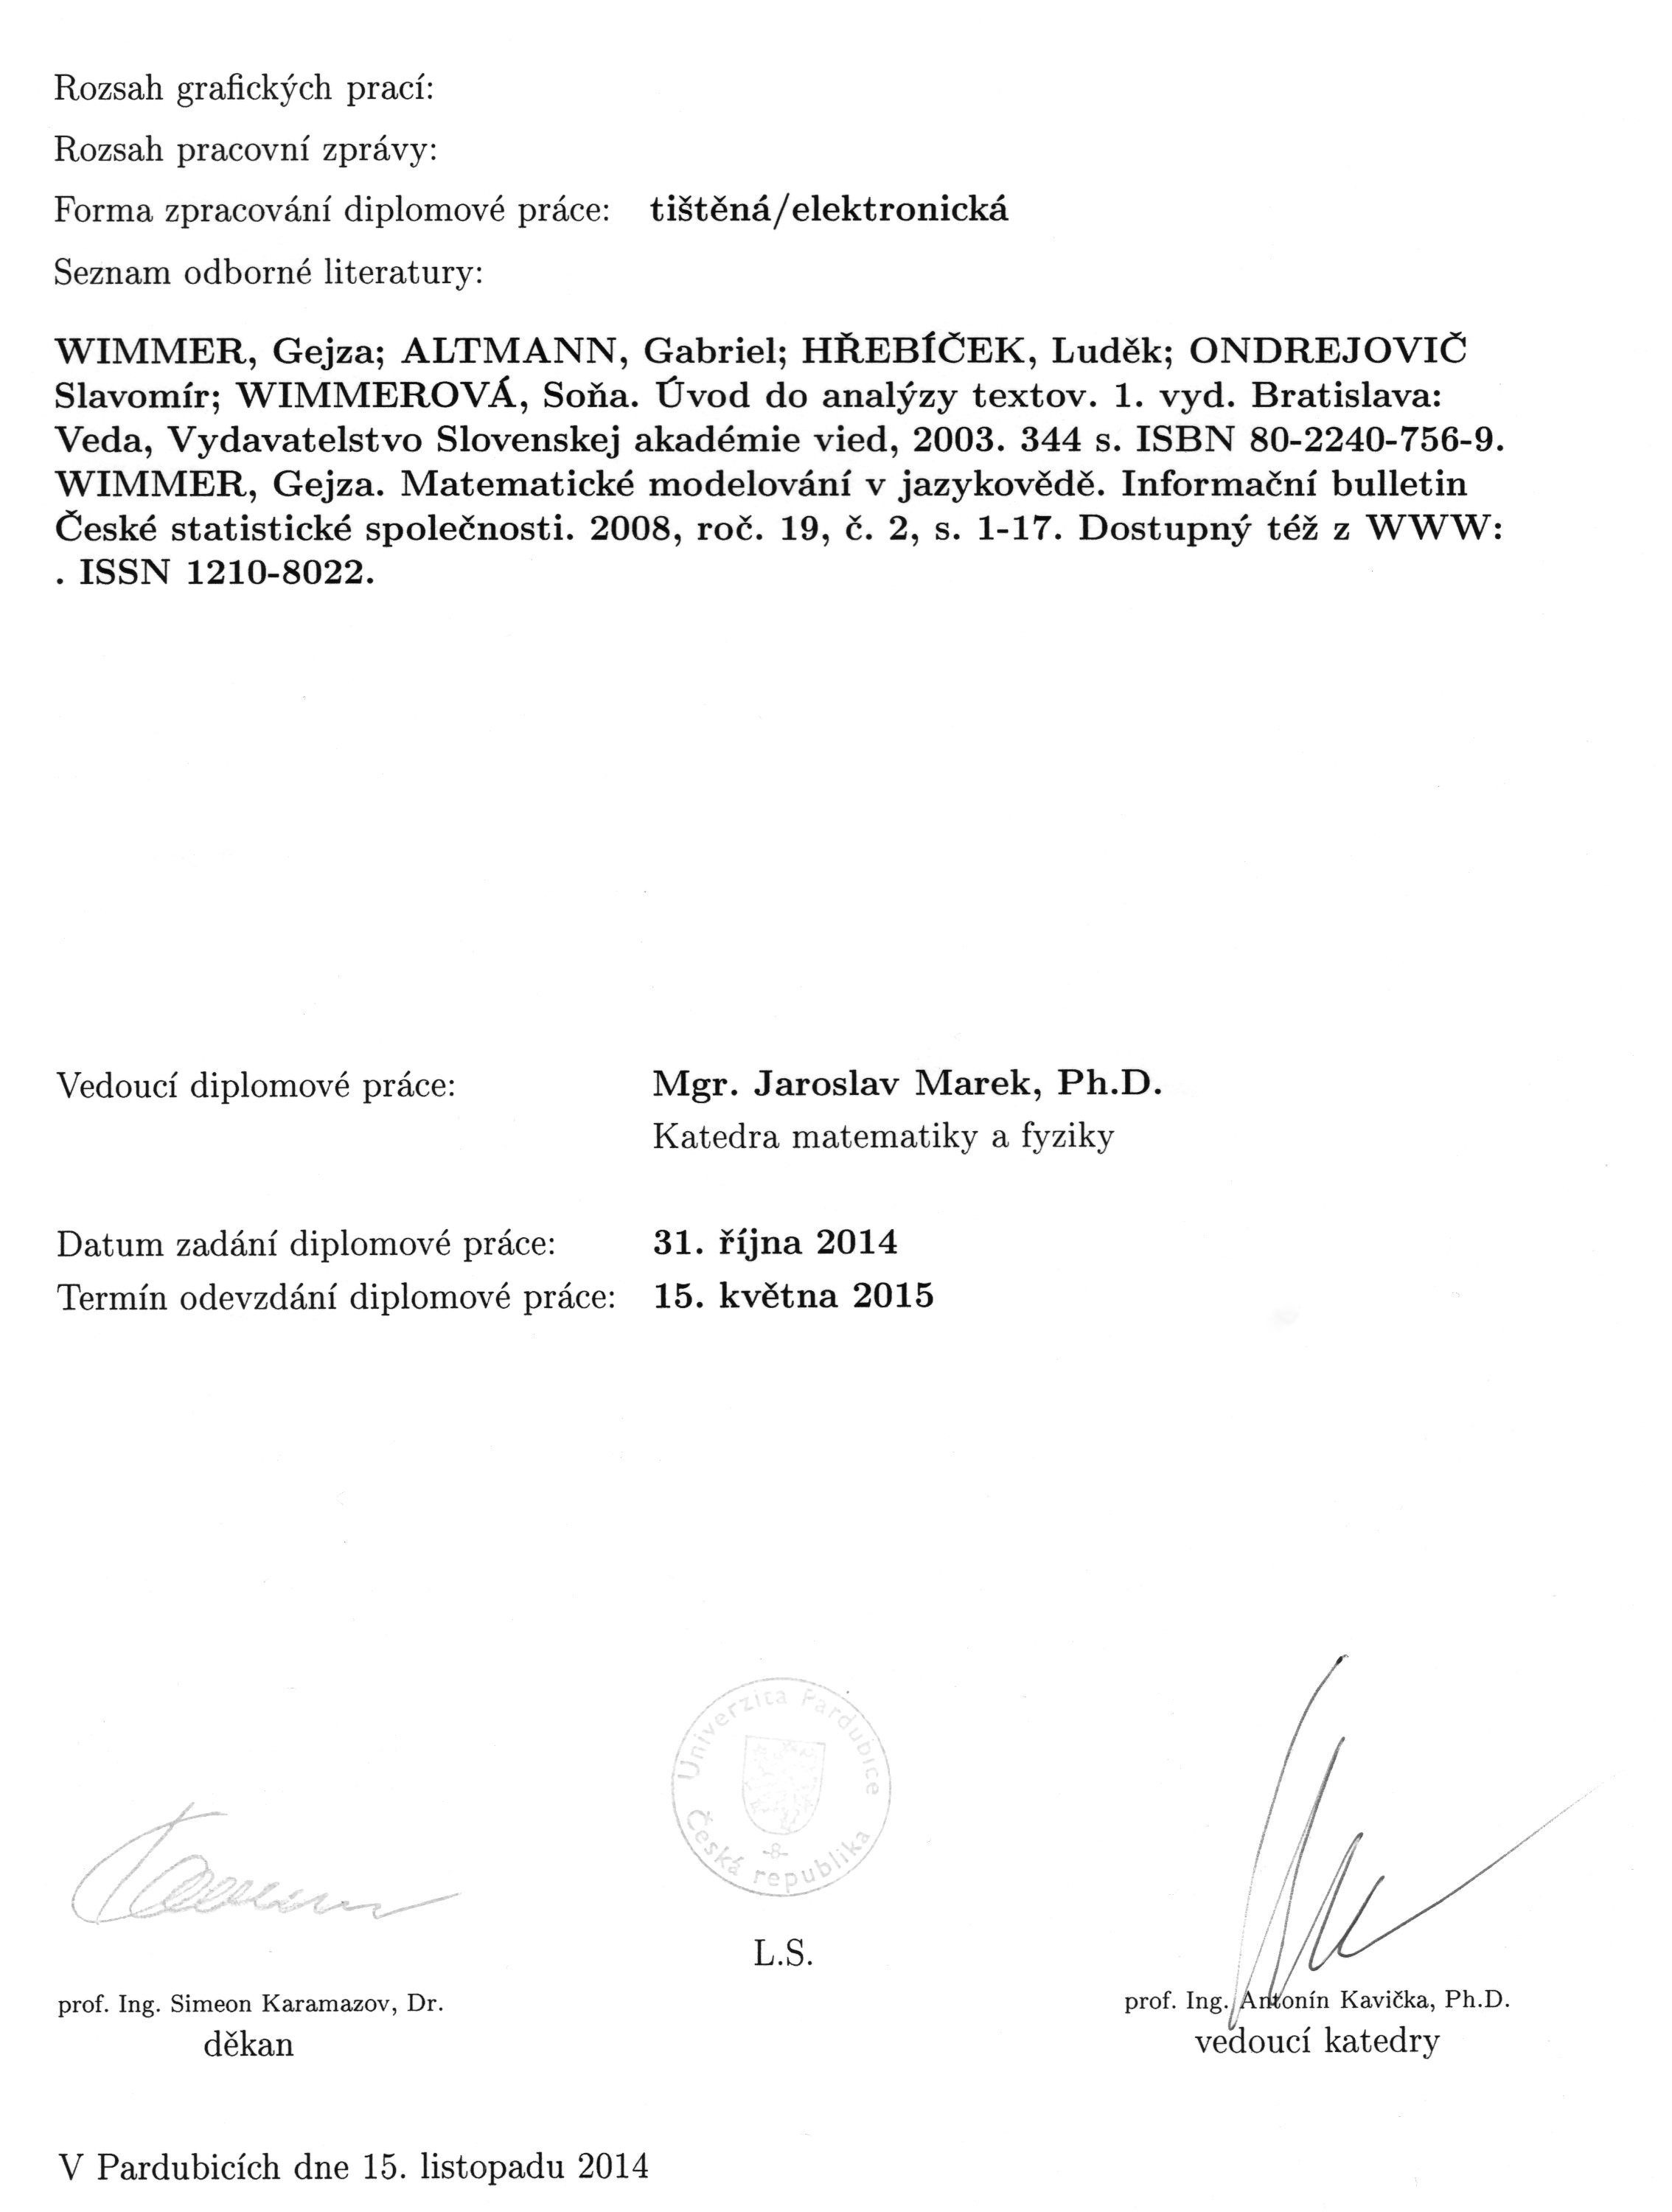
\includegraphics[max width=\textwidth,keepaspectratio=true]{imgs-00-zadani/zadani_str_2.png}
\end{center}
\hspace{0pt}

%\onehalfspacing
\spacing{1.25}

\newpage 
\thispagestyle{empty}
\subsubsection*{Prohlášení autora}

Prohlašuji, že jsem tuto práci vypracoval samostatně. Veškeré literární prameny a informace, které jsem v práci využil, jsou uvedeny v seznamu použité literatury.

Byl jsem seznámen s tím, že se na moji práci vztahují práva a povinnosti vyplývající ze zákona č. 121/2000 Sb., autorský zákon, zejména se skutečností, že Univerzita Pardubice má právo na uzavření licenční smlouvy o užití této práce jako školního díla podle § 60 odst. 1 autorského zákona, a s tím, že pokud dojde k užití této práce mnou nebo bude poskytnuta licence o užití jinému subjektu, je Univerzita Pardubice oprávněna ode mne požadovat přiměřený příspěvek na úhradu nákladů, které na vytvoření díla vynaložila, a to podle okolností až do jejich skutečné výše.

Souhlasím s prezenčním zpřístupněním své práce v Univerzitní knihovně.\\[4cm]
V Pardubicích dne \today\ \hfill{} Jan Šlahora

\newpage 
\thispagestyle{empty}
\subsubsection*{Poděkování}

Na tomto místě můžete poděkovat osobám, které vám byly nápomocny v průběhu zpracování bakalářské práce, které vás podporovaly během studia, atd.

\newpage 
\thispagestyle{empty}
\subsubsection*{Anotace}
Práce se zabývá studiem vybraných modelů používaných v rámci matematické lingvistiky a jejich následnou aplikací na české překlady básně Havran amerického autora Edgara Allena Poea. V~rámci práce byl vyvinut počítačový program, který umožňuje aplikovat popisované metody na libovolné texty a porovnávat výsledky sledovaných charakteristik. Součástí práce je i srovnání výsledků jednotlivých metod pro české překlady Havrana.

\vspace*{0.8cm}\subsubsection*{Klíčová slova} 	 	 		

lingvistika, statistika, denotační analýza, fonetické jevy, teorie grafů

\vspace*{2.8cm}\subsubsection*{Title}
Computational linguistics and translations of E. A. Poe's poem The Raven

\vspace*{0.8cm}\subsubsection*{Annotation}

Morbi fringilla risus ut arcu dapibus viverra ultricies dolor consequat. Fusce tempus ipsum congue sem blandit in suscipit turpis fermentum. Aliquam vel feugiat nisi. Donec mattis, purus eget sodales condimentum, sapien nunc vestibulum est, ac vehicula sem leo nec mi. Sed id luctus nulla. Class aptent taciti sociosqu ad litora torquent per conubia nostra, per inceptos himenaeos. Sed condimentum aliquet lorem in aliquet. Aliquam sed erat mauris. Pellentesque habitant morbi tristiqěue senectus et netus et malesuada fames ac turpis egestas. Nam eu dui in ante posuere pulvinar at vel purus. Phasellus consequat sollicitudin tempus. Ut nec elit nisi. 

\vspace*{0.8cm}\subsubsection*{Keywords}

linguistics, statistics, denotation analysis, phonetic phenomenon, graph theory

\tableofcontents

\let\cleardoublepage\clearpage % vymazání prázdné stránky http://stackoverflow.com/questions/491904/latex-how-to-remove-blank-pages-coming-between-two-chapters-in-appendix

\chapter*{Seznam pojmů a zkratek}
\addcontentsline{toc}{chapter}{Seznam pojmů a zkratek}  

\printglossary[title=Slovník pojmů, nonumberlist]

\printglossary[type=acronym, title=Slovník zkratek, nonumberlist]   

\listoffigures
\addcontentsline{toc}{chapter}{\listfigurename} 

\listoftables
\addcontentsline{toc}{chapter}{\listtablename} 

\thispagestyle{empty}

\subfile{00-predmluva}
\subfile{10-uvod}
\subfile{50-denotacni-analyza}
\subfile{60-aplikace}
\subfile{70-experiment}
\subfile{99-zaver}


\printbibliography[title={Seznam použité literatury},heading=bibintoc]

\appendix
\subfile{99-appendix}


\end{document}